\documentclass[12pt,a4paper]{article}
\usepackage{amsmath,amscd,amsbsy,amssymb,latexsym,url,bm,amsthm}
\usepackage{epsfig,graphicx,subfigure}
\usepackage{enumitem,balance}
\usepackage{wrapfig}
\usepackage{mathrsfs,euscript}
\usepackage[usenames]{xcolor}
\usepackage{hyperref}
\usepackage[vlined,ruled,linesnumbered]{algorithm2e}
\usepackage{array}
\hypersetup{colorlinks=true,linkcolor=black}

\newtheorem{theorem}{Theorem}
\newtheorem{lemma}[theorem]{Lemma}
\newtheorem{proposition}[theorem]{Proposition}
\newtheorem{corollary}[theorem]{Corollary}
\newtheorem{exercise}{Exercise}
\newtheorem*{solution}{Solution}
\newtheorem{definition}{Definition}
\theoremstyle{definition}

\renewcommand{\thefootnote}{\fnsymbol{footnote}}

\newcommand{\postscript}[2]
 {\setlength{\epsfxsize}{#2\hsize}
  \centerline{\epsfbox{#1}}}

\renewcommand{\baselinestretch}{1.0}

\setlength{\oddsidemargin}{-0.365in}
\setlength{\evensidemargin}{-0.365in}
\setlength{\topmargin}{-0.3in}
\setlength{\headheight}{0in}
\setlength{\headsep}{0in}
\setlength{\textheight}{10.1in}
\setlength{\textwidth}{7in}
\makeatletter \renewenvironment{proof}[1][Proof] {\par\pushQED{\qed}\normalfont\topsep6\p@\@plus6\p@\relax\trivlist\item[\hskip\labelsep\bfseries#1\@addpunct{.}]\ignorespaces}{\popQED\endtrivlist\@endpefalse} \makeatother
\makeatletter
\renewenvironment{solution}[1][Solution] {\par\pushQED{\qed}\normalfont\topsep6\p@\@plus6\p@\relax\trivlist\item[\hskip\labelsep\bfseries#1\@addpunct{.}]\ignorespaces}{\popQED\endtrivlist\@endpefalse} \makeatother

\usepackage{tikz}
\usepackage{tcolorbox}
\usepackage{listings}
\definecolor{grey}{rgb}{0.8,0.8,0.8}
\definecolor{darkgreen}{rgb}{0,0.3,0}
\definecolor{darkblue}{rgb}{0,0,0.3}
\lstset{%
    numbers=left, %行号
    numberstyle=\tiny\color{grey},
    showstringspaces=false,
    showspaces=false,%
    tabsize=4,%
    frame=shadowbox,%
    basicstyle={\ttfamily\scriptsize},%
    keywordstyle=\color{blue!80!black}\bfseries,%
    identifierstyle=,%
    commentstyle=\color{green!50!blue}\itshape,%
    stringstyle=\color{green!50!black},%
    rulesepcolor=\color{gray!20!white},
    breaklines,
    columns=flexible,
    extendedchars=false,
    %mathescape=true,
}
\usepackage{multicol}
\setlength{\columnsep}{30pt}


\begin{document}
\noindent

%========================================================================
\noindent\framebox[\linewidth]{\shortstack[c]{
\Large{\textbf{Lab08-Graph Exploration}}\vspace{1mm}\\
CS214-Algorithm and Complexity, Xiaofeng Gao \& Lei Wang, Spring 2021.}}
\begin{center}
\footnotesize{\color{red}$*$ If there is any problem, please contact TA Yihao Xie. }

\footnotesize{\color{blue}$*$ Name: Log Creative  \quad Student ID:  \quad Email: logcreative-lzl@sjtu.edu.cn}
\end{center}

\begin{enumerate}

	\item Given an undirected graph $G = (V, E)$. Prove the following propositions.
	
	\begin{enumerate}
		\item Let $e$ be a maximum-weight edge on some cycle of connected graph $G=(V,E)$.
        Then there is a minimum spanning tree of $G$ that does not include $e$. Moreover, there is no minimum spanning tree of $G$ that includes $e$ if $e$ is the unique maximum-weight edge on the cycle. 
        % \begin{proof}
            \begin{proposition}\label{prop:ni}
                There is a minimum spanning tree of $G$ that does not include $e$.
            \end{proposition}
            \textbf{Proof of Proposition \ref{prop:ni}.} Suppose $e:v_0\leftrightarrow v_1$ is on the cycle 
            \begin{equation*}
                v_0\rightarrow v_1\rightarrow \cdots\rightarrow v_n\rightarrow v_0
            \end{equation*}
            where $n\geq 1$ because there has at least one edge $e$. If there is a minimum spanning tree $T=(V,E_T)$ that include $e$, consider the graph $(V,E_T-\{e\})$, either $v_0$ or $v_1$ is an isolated vertex. Otherwise, $v_0$ and $v_1$ are connected in $G^\prime =(V,E_T-\{e\})$ by a path $l$, with the addition of $\{e\}$ to form the original graph $(V,E_T-\{e\}+\{e\})=T$, there must be a loop:
            \begin{equation*}
                v_0 \stackrel{e}{\longleftrightarrow} v_{1} \stackrel{l}{\longleftrightarrow} v_0
            \end{equation*}
            which conflicts the definition of the tree $T$.

            \begin{figure}[h]
                \centering
                \begin{tikzpicture}[node distance=9pt]
\tikzstyle{blackdot}=[circle,scale=0.3,fill];

\draw (0,-0.5) node [blackdot] (v0) {} -- (1,-1)node [blackdot] (v1) {};
\node[above of=v0] {$v_0$};
\node[right of=v1] {$v_1$};
\node[draw,circle,minimum width=16pt] (v2) at (1,1) {};
\draw  (v2) edge (v1);
\draw  (v0) edge node[above] {$e$} (v1);
\draw (-1.5,0) node[blackdot] (vn) {} edge[dashed] (v0);
\node[above of=vn] {$v_n$};

\draw[dashed]  plot[smooth, tension=.7] coordinates {(v1) (0.5,-2.5) (-1.5,-2.5) (-2.5,-1) (vn)};
\draw  (vn) edge (v2);
\draw  (vn) edge[draw=none] node[above] {$e^\prime$} (v0);
\end{tikzpicture}

                \caption{Diagram for Problem (a)}
                \label{fig:ni}
            \end{figure}

            Without the loss of generality, suppose $v_0$ is the isolated vertex, shown in Figure \ref{fig:ni}. Then consider the edge $e^\prime:v_n\leftrightarrow v_0$ on the loop, $T^\prime = (V,E_T-\{e\}+\{e^\prime\})$ is a spanning tree. Because $v_n$ is connected in $G^\prime =(V,E_T-\{e\})$ because $T$ is a spanning tree and the loss of $\{e\}$ could only damage the connectivity of $v_0$. The operation will reconnect $v_0$.
            
            Due to the maximality of weight for $e$ on the loop,
            \begin{equation*}
                |e^\prime|\leq |e|
            \end{equation*}

            Thus, the new spanning tree will also be a minimum spanning tree derived from
            \begin{equation*}
                \sum_{e_i\in E_T-\{e\}}|e_i| + |e^\prime|\leq|e|+ \sum_{e_i\in E_T-\{e\}}|e_i|
            \end{equation*}
            where $T^\prime=(V,E_T-\{e\}+\{e^\prime\})$ does not include $e$.

            % then the tree could not contain all the edges on the loop, otherwise it will conflict the definition of a tree. Suppose it does not contain the edge $e^\prime$ on the loop, then because $e$ is the maximum-weight edge on the loop,
            % \begin{equation*}
            %     |e^\prime|\leq |e|
            % \end{equation*}
            % Hence, the $e$ could be substituted by $e^\prime$ in the minimum spanning tree and contruct a new tree $T^\prime=(V,E_T-\{e\}+\{e^\prime\})$, with the sum of weight suffies
            % \begin{equation*}
            %     \sum_{e_i\in E_T-\{e\}}|e_i| + |e^\prime|\leq|e|+ \sum_{e_i\in E_T-\{e\}}|e_i|
            % \end{equation*}
            % which indicates that $T^\prime$ is also a minimum spanning tree.

            % Such a substitution $e^\prime$ could always be properly found. By contradiction, for all missing edges $e^\prime_j: v_j\leftrightarrow v_{j+1}$ on the loop in the tree $T$, if $T^{\prime\prime}=(V,E_T-\{e\}+\{e^\prime_j\})$ could always form anothor loop
            % \begin{equation*}
            %     v_j \stackrel{e}{\longleftrightarrow} v_{j+1} \stackrel{l}{\longrightarrow} v_j
            % \end{equation*}
            % where $l$ is a path from $v_{j+1}$ to $v_j$. Then, removing all the edges on the path $l$ from tree , and add $e$ to the graph will not change the connectivity of 
            
            \hfil \qed \vspace{\parskip}
            
            \begin{proposition}\label{prop:ns}
                There is no minimum spanning tree that includes $e$ if such weight on $e$ is unique.
            \end{proposition}
            \textbf{Proof of Proposition \ref{prop:ns}.} 
                Proof by contradiction. Suppose the minimum spanning tree $T$ contains $e$, then by the same deduction in Proposition \ref{prop:ni}, the weight of $e^\prime: v_n\leftrightarrow v_0$ is strictly smaller than that of $e$.
                \begin{equation*}
                    |e^\prime|< |e|
                \end{equation*}
                Thus, the new spanning tree $T^\prime=(V,E-\{e\}+\{e^\prime\})$ will get a smaller overall weight of edges.
                \begin{equation*}
                    \sum_{e_i\in E_T-\{e\}}|e_i| + |e^\prime| < |e|+ \sum_{e_i\in E_T-\{e\}}|e_i|
                \end{equation*}
                which conflicts the minimality of $T$. Therefore, the minimum spanning tree does not include $e$ in this scenario.
            \hfil \qed \vspace{\parskip}
        % \end{proof}
		\item Let $T$ and $T'$ are two different minimum spanning trees of $G$. Then $T'$ can be obtained from $T$ by repeatly substitute one edge in $T\backslash T'$ by one edge in $T'\backslash T$ and meanwhile the result after each subsitution is still a minimum spanning tree.
		\begin{proof}
            Because $T$ and $T^\prime$ share the same set of vertices $V$ of $G$, the property of spanning tree will guarantee that 
            \begin{equation}\label{eq:ne}
                |E_T| = |E_{T^\prime}| = |V|-1
            \end{equation}
            Because $T$ and $T^\prime$ are different, $T\backslash T^\prime,T^\prime\backslash T\neq \varnothing$. The quantity relationship
            \begin{align*}
                |E_T| &= |E_T\cap E_{T^\prime}| + |E_T\backslash E_{T^\prime}|\\
                |E_{T^\prime}| &= |E_T\cap E_{T^\prime}| + |E_{T^\prime}\backslash E_T|
            \end{align*}
            with Equation \eqref{eq:ne} follows that 
            \begin{equation}\label{eq:eq}
                |E_T\backslash E_{T^\prime}| = |E_{T^\prime}\backslash E_T|\neq 0
            \end{equation}
            Thus, there always exists $e\in T\backslash T^\prime$, where $e:v_0\leftrightarrow v_1$. Because $e\not\in T^\prime\backslash T$ and there is no loop in $T$, suppose $v_0$ is isolated in $(V,E_T-\{e\})$. $T^\prime \backslash T$ must come up with a path $l\subseteq E_{T^\prime}\backslash E_T$ to connect $v_0\stackrel{l}{\longleftrightarrow}v_1$. As a consequence, there is a loop in $G$.
            \begin{equation*}
                v_0 \stackrel{e}{\longleftrightarrow} v_{1} \stackrel{l}{\longleftrightarrow} v_0
            \end{equation*}
            Similar to the construction in Proposition \ref{prop:ni}, $e^\prime(v_n\leftrightarrow v_0)\in l$ could be selected. 
            
            \begin{figure}[h]
                \centering
                \begin{tikzpicture}[node distance=9pt]
\tikzstyle{blackdot}=[circle,scale=0.3,fill];

\draw[draw=red] (0,-0.5) node [blackdot] (v0) {} -- (1,-1)node [blackdot] (v1) {};
\node[above of=v0] {$v_0$};
\node[right of=v1] {$v_1$};
\node[draw,circle,minimum width=16pt,red] (v2) at (1,1) {$T$};
\draw[red]  (v2) edge (v1);
\draw[red]  (v0) edge node[above] {$e$} (v1);
\draw (-1.5,0) node[blackdot] (vn) {} edge[dashed,draw=none] (v0);
\node[above of=vn,red] {$v_n$};

%\draw[dashed,blue]  plot[smooth, tension=.7] coordinates {(v1) (0.5,-2.5) (-2,-2.5) (-2.5,-1) (vn)};
\draw[red]  (vn) edge (v2);
\draw[blue]  (vn) edge[draw=none] node[above] {$e^\prime$} (v0);
\node[draw,circle,minimum width=16pt,blue] (v2) at (-1.5,-2) {$T^\prime$};
\draw[blue]  (v2) edge (vn);
\draw[blue]  (v2) edge (v1);
\draw[blue]  (v0) edge (vn);
\end{tikzpicture}
                \caption{Diagram for Problem (b)}
                \label{fig:db}
            \end{figure}

            Shown in Figure \ref{fig:db}, if $|e^\prime|<|e|$, the new spanning tree $(V,E_T-\{e\}+\{e^\prime\})$ will be even smaller than $T$, which violates the minimality of $T$. If $|e^\prime|>|e|$, the spanning tree $(V,E_{T^\prime}-\{e^\prime\}+\{e\})$ will be even smaller than $T^\prime$, which also violates the minimality of $T^\prime$. Therefore, $|e^\prime|=|e|$. This procedure will not damage the minimality of the new spanning tree and equation \eqref{eq:eq} guarantees that the subsitution will always exists.
            % $\not\exists e^{\prime\prime}(v_0\leftrightarrow v_1)\in E_T\cap E_{T^\prime}$
        \end{proof}
	\end{enumerate}
	
    \item Let $G=(V,E)$ be a connected, undirected graph. Give an $O(|V|+|E|)$-time algorithm
    to compute a path in $G$ that traverses each edge in $E$ exactly once in each direction. Describe how you can find your way out of a maze if you are given enough coins to apply your algorithm.

    \begin{solution}

        The implementation is shown in Algorithm \ref{alg:td} to traverse each edge in $E$ exactly once in each direction. 
        
        \paragraph{Explanation.} The modified DFS shown in Function \texttt{DFS} will record the previous point of the process. After starting from the edge, the starting vertex will be recorded as visited in Line \textbf{2}. After leaving the vertex, the ending vertex will also be recorded as visited in Line \textbf{14}. 
        Because the process is trigged from $e$, the early turnback on edge $e$ is not allowed in Line \textbf{5}.
        If the adjacent vertex is visited before but the edge is not, then the path will make a loop to traverse exactly both directions of the edge in Line \textbf{9}. If it is not visited, the DFS process will start from the unvisited adjacent vertex in Line \textbf{12}. An executing example is shown in Figure \ref{fig:exe}.
        
        \begin{figure}[h]
            \centering
            \subfigure[1]{\begin{tikzpicture}
\tikzstyle{blackdot}=[circle,scale=0.3,fill];
\node [blackdot,red] (v2) at (-0.5,0.5) {};
\node [blackdot] (v1) at (-1.5,-1) {};
\node [blackdot] (v3) at (0.5,-1) {};
\draw  (v1) edge[bend left] (v2);
\draw  (v2) edge[bend left] (v1);
\draw  (v3) edge (v2);
\draw  (v1) edge (v3);
\draw  (v2) edge[loop, looseness=20] (v2);
\node [blackdot] (v4) at (-0.5,-0.5) {};
\draw  (v3) edge (v4);
\end{tikzpicture}
}
            \subfigure[$\rightarrow$1$\rightarrow$1]{\begin{tikzpicture}
\tikzstyle{blackdot}=[circle,scale=0.3,fill];
\node [blackdot,red] (v2) at (-0.5,0.5) {};
\node [blackdot] (v1) at (-1.5,-1) {};
\node [blackdot] (v3) at (0.5,-1) {};
\draw  (v1) edge[bend left] (v2);
\draw  (v2) edge[bend left] (v1);
\draw  (v3) edge (v2);
\draw  (v1) edge (v3);
\draw  (v2) edge[loop, looseness=20,red,thick] (v2);
\node [blackdot] (v4) at (-0.5,-0.5) {};
\draw  (v3) edge (v4);
\end{tikzpicture}}
            \subfigure[$\rightarrow$]{\begin{tikzpicture}
\tikzstyle{blackdot}=[circle,scale=0.3,fill];
\node [blackdot,red] (v2) at (-0.5,0.5) {};
\node [blackdot] (v1) at (-1.5,-1) {};
\node [blackdot] (v3) at (0.5,-1) {};
\draw  (v1) edge[red,bend left] (v2);
\draw  (v2) edge[bend left] (v1);
\draw  (v3) edge (v2);
\draw  (v1) edge (v3);
\draw  (v2) edge[loop, looseness=20,red,thick] (v2);
\node [blackdot] (v4) at (-0.5,-0.5) {};
\draw  (v3) edge (v4);
\end{tikzpicture}
}
            \subfigure[2$\rightarrow$1$\rightarrow$2]{\begin{tikzpicture}
\tikzstyle{blackdot}=[circle,scale=0.3,fill];
\node [blackdot,red] (v2) at (-0.5,0.5) {};
\node [blackdot,red] (v1) at (-1.5,-1) {};
\node [blackdot] (v3) at (0.5,-1) {};
\draw  (v1) edge[red,bend left] (v2);
\draw  (v2) edge[red,bend left,thick] (v1);
\draw  (v3) edge (v2);
\draw  (v1) edge (v3);
\draw  (v2) edge[loop, looseness=20,red,thick] (v2);
\node [blackdot] (v4) at (-0.5,-0.5) {};
\draw  (v3) edge (v4);
\end{tikzpicture}}
            \subfigure[$\rightarrow$]{\begin{tikzpicture}
\tikzstyle{blackdot}=[circle,scale=0.3,fill];
\node [blackdot,red] (v2) at (-0.5,0.5) {};
\node [blackdot,red] (v1) at (-1.5,-1) {};
\node [blackdot] (v3) at (0.5,-1) {};
\draw  (v1) edge[red,bend left] (v2);
\draw  (v2) edge[red,bend left,thick] (v1);
\draw  (v3) edge (v2);
\draw  (v1) edge[red] (v3);
\draw  (v2) edge[loop, looseness=20,red,thick] (v2);
\node [blackdot] (v4) at (-0.5,-0.5) {};
\draw  (v3) edge (v4);
\end{tikzpicture}
}

            \subfigure[3$\rightarrow$]{\begin{tikzpicture}
\tikzstyle{blackdot}=[circle,scale=0.3,fill];
\node [blackdot,red] (v2) at (-0.5,0.5) {};
\node [blackdot,red] (v1) at (-1.5,-1) {};
\node [blackdot,red] (v3) at (0.5,-1) {};
\draw  (v1) edge[red,bend left] (v2);
\draw  (v2) edge[red,bend left,thick] (v1);
\draw  (v3) edge (v2);
\draw  (v1) edge[red] (v3);
\draw  (v2) edge[loop, looseness=20,red,thick] (v2);
\node [blackdot] (v4) at (-0.5,-0.5) {};
\draw  (v3) edge[red] (v4);
\end{tikzpicture}
}
            \subfigure[4$\rightarrow$3]{\begin{tikzpicture}
\tikzstyle{blackdot}=[circle,scale=0.3,fill];
\node [blackdot,red] (v2) at (-0.5,0.5) {};
\node [blackdot,red] (v1) at (-1.5,-1) {};
\node [blackdot,red] (v3) at (0.5,-1) {};
\draw  (v1) edge[red,bend left] (v2);
\draw  (v2) edge[red,bend left,thick] (v1);
\draw  (v3) edge (v2);
\draw  (v1) edge[red] (v3);
\draw  (v2) edge[loop, looseness=20,red,thick] (v2);
\node [blackdot,red] (v4) at (-0.5,-0.5) {};
\draw  (v3) edge[red,thick] (v4);
\end{tikzpicture}}
            \subfigure[$\rightarrow$1$\rightarrow$3]{\begin{tikzpicture}
\tikzstyle{blackdot}=[circle,scale=0.3,fill];
\node [blackdot,red] (v2) at (-0.5,0.5) {};
\node [blackdot,red] (v1) at (-1.5,-1) {};
\node [blackdot,red] (v3) at (0.5,-1) {};
\draw  (v1) edge[red,bend left] (v2);
\draw  (v2) edge[red,bend left,thick] (v1);
\draw  (v3) edge[red,thick] (v2);
\draw  (v1) edge[red] (v3);
\draw  (v2) edge[loop, looseness=20,red,thick] (v2);
\node [blackdot,red] (v4) at (-0.5,-0.5) {};
\draw  (v3) edge[red,thick] (v4);
\end{tikzpicture}
}
            \subfigure[$\rightarrow$2]{\begin{tikzpicture}
\tikzstyle{blackdot}=[circle,scale=0.3,fill];
\node [blackdot,red] (v2) at (-0.5,0.5) {};
\node [blackdot,red] (v1) at (-1.5,-1) {};
\node [blackdot,red] (v3) at (0.5,-1) {};
\draw  (v1) edge[red,bend left] (v2);
\draw  (v2) edge[red,bend left,thick] (v1);
\draw  (v3) edge[red,thick] (v2);
\draw  (v1) edge[red,thick] (v3);
\draw  (v2) edge[loop, looseness=20,red,thick] (v2);
\node [blackdot,red] (v4) at (-0.5,-0.5) {};
\draw  (v3) edge[red,thick] (v4);
\end{tikzpicture}}
            \subfigure[$\rightarrow$1]{\begin{tikzpicture}
\tikzstyle{blackdot}=[circle,scale=0.3,fill];
\node [blackdot,red] (v2) at (-0.5,0.5) {};
\node [blackdot,red] (v1) at (-1.5,-1) {};
\node [blackdot,red] (v3) at (0.5,-1) {};
\draw  (v1) edge[red,bend left,thick] (v2);
\draw  (v2) edge[red,bend left,thick] (v1);
\draw  (v3) edge[red,thick] (v2);
\draw  (v1) edge[red,thick] (v3);
\draw  (v2) edge[loop, looseness=20,red,thick] (v2);
\node [blackdot,red] (v4) at (-0.5,-0.5) {};
\draw  (v3) edge[red,thick] (v4);
\end{tikzpicture}
}
            \caption{An excuting example.}
            \label{fig:exe}
        \end{figure}
        
        \paragraph{Correctness.} It uses a $second$ matrix to store the edge that has been visited, which makes sure that if the edge is visited twice, it can not be visited again. If it is in the procedure of visiting $e$, it can not be visited backwards until the local DFS is finished. DFS has been proved that every connected vertices will be visited in the connected $G$. If there is an edge $e^\prime$ that hasn't been visited after the traverse, where the edge $e^\prime$ connects $v$ and $v^\prime$. Then $v$ must been visited due to a connected graph, the edge connect to it must be visited if $second[e]$ is false. And initially, all edge is set to false. A contradiction indicates that all edges are visited.
        
        \paragraph{Time Complexity.} The time complexity is analyzed as follows:
        \begin{description}
            \item[Initialization.] Clearing the vertex visited array $first[v]$ costs $O(|V|)$. Clearing the edge visited matrix $second[e]$ costs $O(|E|)$.
            \item[DFS.] The depth-first search has a running time of $O(|V|+|E|)$, which is shown in Function \texttt{DFS}.
        \end{description}
        As a result, the total running time is $O(|V|+|E|)$.

        To find a way out of a maze, the use of optional parameter $f$ in \texttt{DFS} is necessary. When the path hits the finish point, the whole \texttt{DFS} process will stop and return the path to the finish point. The implementation is shown in Algorithm \ref{alg:maze}.
    \begin{function}[!htbp]
        \caption{DFS($G$,$s$,$t$,$e$=\texttt{NULL},$f=$\texttt{NULL})}
        \KwData{Graph $G$, the source vertex $s$, the target vertex $t$, the optional finsh point $f$}
        \KwOut{Path segement $l$ from and back to $s$, or the path to $f$}
        \BlankLine
        % \lIf(){$e=$\texttt{NULL}}{
            $l\leftarrow (s)$\;
        % }
        %\lElse(){$l\leftarrow (s\stackrel{e}{\rightarrow}t)$}
        $first[s]\leftarrow true$\;
        \ForEach(){$e_i$ in $adj(t)$}{
            $v\leftarrow$ the other end of $e$\;
            \lIf(){$e_i=e$}{\textbf{continue}}
            \lIf(){$v=f$}{\Return{$l\leftarrow (l\stackrel{e}{\rightarrow}t \stackrel{e_i}{\rightarrow} f)$}}
            \If(){$first[v]=true$}{
                \If(){$second[e_i]=false$}{ $l\leftarrow (l \stackrel{e_i}{\rightarrow} v\stackrel{e_i}{\rightarrow} t)$\;
                $second[e_i]\leftarrow true$\;
                }
            }
            \Else{
                $l\leftarrow (l \stackrel{e}{\rightarrow}$\DFS($t$,$v$,$e_i$))\;
                \lIf(){end of $l$=$f$}{
                    \Return{$l$}
                }
            }
        }
        $first[t]\leftarrow true$\;
        $l\leftarrow (l\stackrel{e}{\rightarrow} s)$\;
        \Return{$l$}\;
    \end{function}
    \begin{algorithm}[!htbp]
        \caption{Traverse each edge in both direction}
        \label{alg:td}
        \KwIn{Graph $G=(V,E)$}
        \KwOut{The path that traverses every edge in $G$ exactly once in each direction}
        \BlankLine
        \ForEach(){$v\in V$}{
            $first[v]\leftarrow false$\;
        }
        \ForEach(){$e\in E$}{
            $second[e]\leftarrow false$\;
        }
        choose an edge $v_0\in V$ randomly\;
        \Return{\DFS$(G,v_0,v_0,\texttt{NULL})$}\;
    \end{algorithm}
    \begin{algorithm}[!htbp]
        \caption{Find a way out of a maze}
        \label{alg:maze}
        \KwIn{Maze $G=(V,E)$, Begin $b$, Finish $f$}
        \KwOut{The path $l$ from $b$ to $f$}
        \BlankLine
        \ForEach(){$v\in V$}{
            $first[v]\leftarrow false$\;
        }
        \ForEach(){$e\in E$}{
            $second[e]\leftarrow false$\;
        }
        \Return{\DFS$(G,b,b,\texttt{NULL},f)$}\;
    \end{algorithm}
    \end{solution}

    \item Consider the maze shown in Figure \ref{Fig-Maze}. The black blocks in the figure are blocks that can not be passed through. Suppose the block are explored in the order of right, down, left and up. That is, to go to the next block from $(X,Y)$, we always explore $(X,Y+1)$ first, and then $(X+1,Y)$,$(X,Y-1)$ and$(X-1,Y)$ at last. Answer the following subquestions:
    \begin{figure}[!htbp]
        \centering
        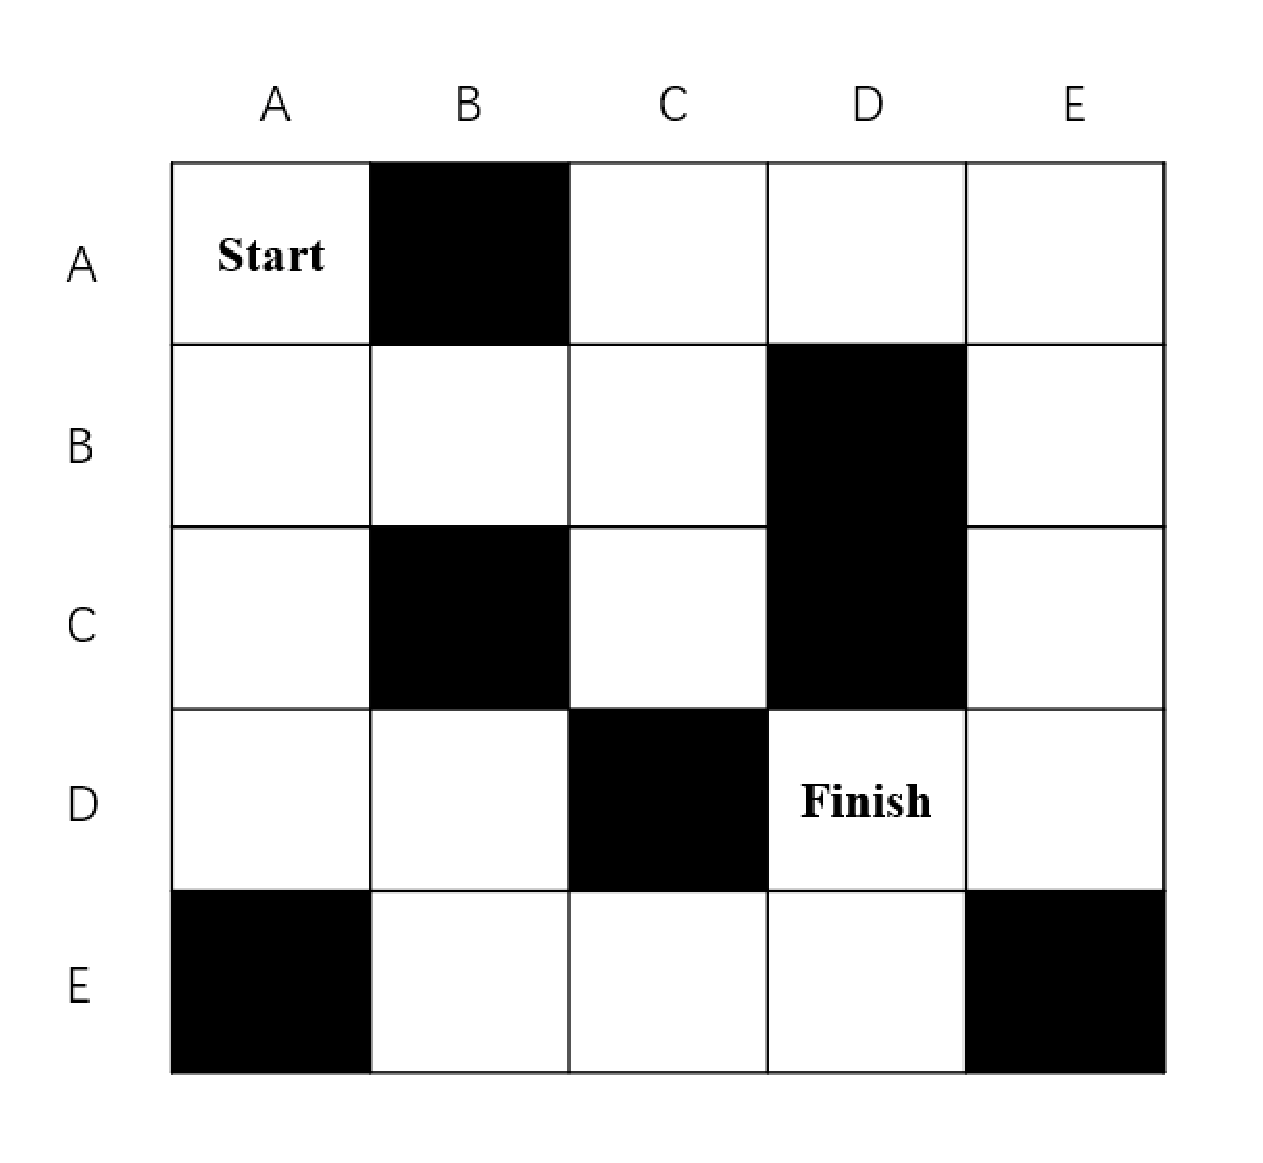
\includegraphics[width=0.45\textwidth]{Fig-Maze.pdf}
        \caption{The blocks in the maze.}
        \label{Fig-Maze}
    \end{figure}
    \begin{enumerate}
        \item Give the sequence of the blocks explored by using DFS to find a path from the ``start" to the ``finish".
        \begin{solution}
            The DFS order is:
            \begin{tcolorbox}
                AA, AB, BB, CB, CC, CA, DA, EA, EB, EC, ED, DD
            \end{tcolorbox}
            which is shown in Figure \ref{fig:dfs}.

            And the path found is:
            \begin{tcolorbox}
                AA, AB, BB, CB, CA, DA, EA, EB, EC, ED, DD
            \end{tcolorbox}

            \begin{figure}[h]
                \centering
                \begin{tikzpicture}
\tikzstyle{rect}=[minimum width=1cm,minimum height=1cm,draw];
\tikzstyle{block}=[rect,fill=black];
\tikzstyle{visit}=[rect,fill=gray!20];
\draw[help lines]  (-2,1) grid (3,-4);
\node [block] at (-0.5,0.5) {};
\node [block] at (-0.5,-1.5) {};
\node [block] at (0.5,-2.5) {};
\node [block] at (1.5,-1.5) {};
\node [block] at (1.5,-0.5) {};
\node [block] at (2.5,-3.5) {};
\node [block] at (-1.5,-3.5) {};
\node at (-1.5,1.5) {A};
\node at (-0.5,1.5) {B};
\node at (0.5,1.5) {C};
\node at (1.5,1.5) {D};
\node at (2.5,1.5) {E};
\node at (-2.5,0.5) {A};
\node at (-2.5,-0.5) {B};
\node at (-2.5,-1.5) {C};
\node at (-2.5,-2.5) {D};
\node at (-2.5,-3.5) {E};

\node [visit,font=\bfseries\color{red},draw=red,fill=red!20] at (-1.5,0.5) {1};
\node [visit] at (-1.5,-0.5) {2};
\node [visit] at (-0.5,-0.5) {3};
\node [visit] at (0.5,-0.5) {4};
\node [visit,fill opacity=0.3] at (0.5,-1.5) {5};
\node [visit] at (0.5,0.5) {6};
\node [visit] at (1.5,0.5) {7};
\node [visit] at (2.5,0.5) {8};
\node [visit] at (2.5,-0.5) {9};
\node [visit] at (2.5,-1.5) {10};
\node [visit] at (2.5,-2.5) {11};
\node [visit,font=\bfseries\color{red},draw=red,fill=red!20] at (1.5,-2.5) {12};
\end{tikzpicture}

                \caption{DFS Explored Sequence}
                \label{fig:dfs}
            \end{figure}
            
        \end{solution}
        \item Give the sequence of the blocks explored by using BFS to find the \underline{shortest} path from the ``start" to the ``finish".
        \begin{solution}
            The BFS order is:
            \begin{tcolorbox}
                AA, AB, BB, AC, CB, AD, CC, CA, BD, DA, BE, EA, CE, EB, DE, EC, DD
            \end{tcolorbox}
            which is shown in Figure \ref{fig:bfs}.

            And the shortest path is:
            \begin{tcolorbox}
                AA, AB, AC, AD, BD, BE, CE, DE, DD
            \end{tcolorbox}

            \begin{figure}[h]
                \centering
                \begin{tikzpicture}
\tikzstyle{rect}=[minimum width=1cm,minimum height=1cm,draw];
\tikzstyle{block}=[rect,fill=black];
\tikzstyle{visit}=[rect,fill=gray!20];
\draw[help lines]  (-2,1) grid (3,-4);
\node [block] at (-0.5,0.5) {};
\node [block] at (-0.5,-1.5) {};
\node [block] at (0.5,-2.5) {};
\node [block] at (1.5,-1.5) {};
\node [block] at (1.5,-0.5) {};
\node [block] at (2.5,-3.5) {};
\node [block] at (-1.5,-3.5) {};
\node at (-1.5,1.5) {A};
\node at (-0.5,1.5) {B};
\node at (0.5,1.5) {C};
\node at (1.5,1.5) {D};
\node at (2.5,1.5) {E};
\node at (-2.5,0.5) {A};
\node at (-2.5,-0.5) {B};
\node at (-2.5,-1.5) {C};
\node at (-2.5,-2.5) {D};
\node at (-2.5,-3.5) {E};

\node [visit,font=\bfseries\color{red},draw=red,fill=red!20] at (-1.5,0.5) {1};
\node [visit,font=\bfseries\color{red},draw=red,fill=red!20] at (1.5,-2.5) {17};
\node [visit] at (-1.5,-0.5) {2};
\node [visit,fill opacity=0.3] at (-0.5,-0.5) {3};
\node [visit] at (-1.5,-1.5) {4};
\node [visit,fill opacity=0.3] at (0.5,-0.5) {5};
\node [visit] at (-1.5,-2.5) {6};
\node [visit,fill opacity=0.3] at (0.5,-1.5) {7};
\node [visit,fill opacity=0.3] at (0.5,0.5) {8};
\node [visit] at (-0.5,-2.5) {9};
\node [visit,fill opacity=0.3] at (1.5,0.5) {10};
\node [visit] at (-0.5,-3.5) {11};
\node [visit,fill opacity=0.3] at (2.5,0.5) {12};
\node [visit] at (0.5,-3.5) {13};
\node [visit,fill opacity=0.3] at (2.5,-0.5) {14};
\node [visit] at (1.5,-3.5) {15};
\node [visit,fill opacity=0.3] at (2.5,-1.5) {16};
\end{tikzpicture}
                \caption{BFS Explored Sequence}
                \label{fig:bfs}
            \end{figure}
        \end{solution}
        \item Consider a maze with a larger size. Discuss which of BFS and DFS will be used to find one path and which will be used to find the shortest path from the start block to the finish block.
        \begin{solution}
            \begin{description}
                \item[DFS will be used to find one path.] DFS could reach every connected node, which is proved in the lecture. Then, DFS will certainly find a path that reaches the \textbf{Finish} from \textbf{Start}.
                \item[BFS will be used to find the shortest path.] When \textsc{Eject} happens, BFS will \textsc{Inject} the node unvisited and adjacent to the ejected node with 1 increment on the distance. 
                
                By mathematical induction, the node with distance $d$ will be ejected and the following nodes with distance $d+1$ will be injected, with the basic step starting from $d=0$ where there is only the \textbf{Start} in the queue. Figure \ref{fig:bfsl} shows the process.

                \begin{figure}[h]
                    \centering
                    \begin{tikzpicture}
\tikzstyle{rect}=[minimum width=1cm,minimum height=1cm,draw];
\tikzstyle{block}=[rect,fill=black];
\tikzstyle{visit}=[rect,fill=gray!20];

\node [visit] (v2) at (-2,0.5) {3};
\node [visit] (v1) at (-1,0.5) {4};
\node [above of=v1] {$d$=2};
\node [above of=v2] {$d$=2};

\node [rect,opacity=0.5] (v3) at (0,0.5) {5};
\node [rect,opacity=0.5] (v4) at (1,0.5) {6};
\node [above of=v3] {$d$=3};
\draw[->] (v2) -- (-2,-1) -- (0,-1) -- (v3);
\node at (-1,-1.5) {$++d$};
\end{tikzpicture}
                    \caption{\textsc{Inject}}
                    \label{fig:bfsl}
                \end{figure}
                
                Then nodes are ordered by the distance to \textsc{Inject} to the queue and \textsc{Eject} from the queue. Then before \textbf{Finish} is \textsc{Inject} to the queue, there is no shorter path to \textbf{Finish}. And after \textbf{Finsh} is \textsc{Eject} from the queue, the path is always farther than the path when injected.

                Thus, BFS will find the shortest path from \textbf{Start} to \textbf{Finish}.
                
            \end{description}
        \end{solution}
    \end{enumerate}
	
	\item Given a directed graph $G$, whose vertices and edges information are introduced in data file ``SCC.in". Please find its number of Strongly Connected Components with respect to the following subquestions.
    
    \begin{enumerate}
    	\item Read the code and explanations of the provided C/C++ source code ``SCC.cpp", and try to complete this implementation.
    	\begin{solution}
            The count of Strong Connected Components is
            \begin{tcolorbox}
                \input{SCC.out}
            \end{tcolorbox}
        \end{solution}
    	\item Visualize the above selected Strongly Connected Components for this graph $G$. Use the $Gephi$ or other software you preferred to draw the graph. {\color{blue}(If you feel that the data provided in ``SCC.in'' is not beautiful, you can also generate your own data with more vertices and edges than $G$ and draw an additional graph. Notice that results of your visualization will be taken into the consideration of Best Lab.)}
    	\begin{solution}
            The visualization using Gephi is shown in Figure \ref{fig:gephi}.
            \begin{figure}[h]
                \centering
                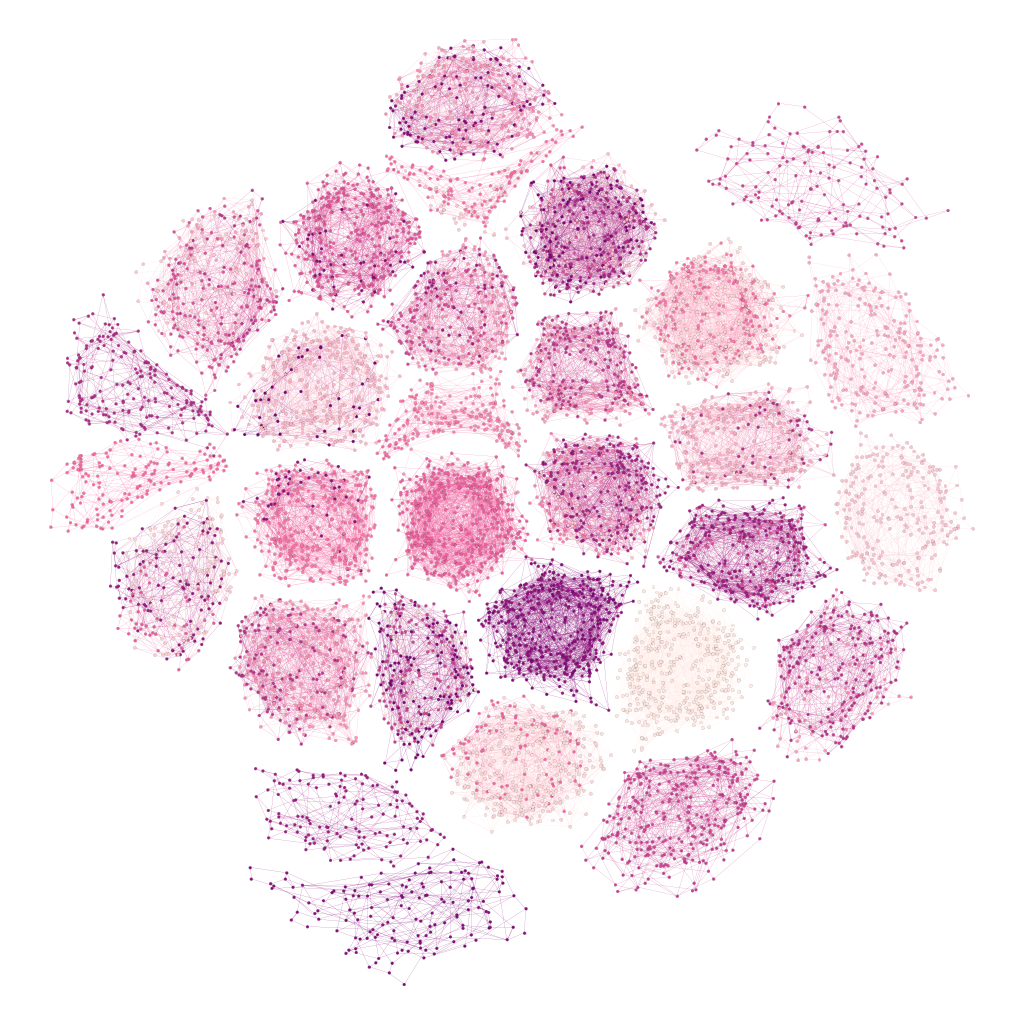
\includegraphics[width=0.4\textwidth]{img/ZilongLi1.png}
                \caption{Using Gephi}
                \label{fig:gephi}
            \end{figure}

            Additionally, the project that I completed in the Principles and Practice of Problem Solving course is also used to visualize the graph. GraphGenDecomp program visualize the Strong Connected Components (SCC) and all edges in Figure \ref{fig:ggd}. You can get more information about this program on \href{https://github.com/LogCreative/GraphGenDecomp/blob/master/report/GraphGenDecomp.pdf}{GraphGenDecomp on GitHub}, which is implemented in C++ and Fast Light Toolkit (FLTK). Basically, it uses spiral funciton to organize nodes into a centralized form for every sub-graph.
            \begin{figure}[h]
                \subfigure[SCC only]{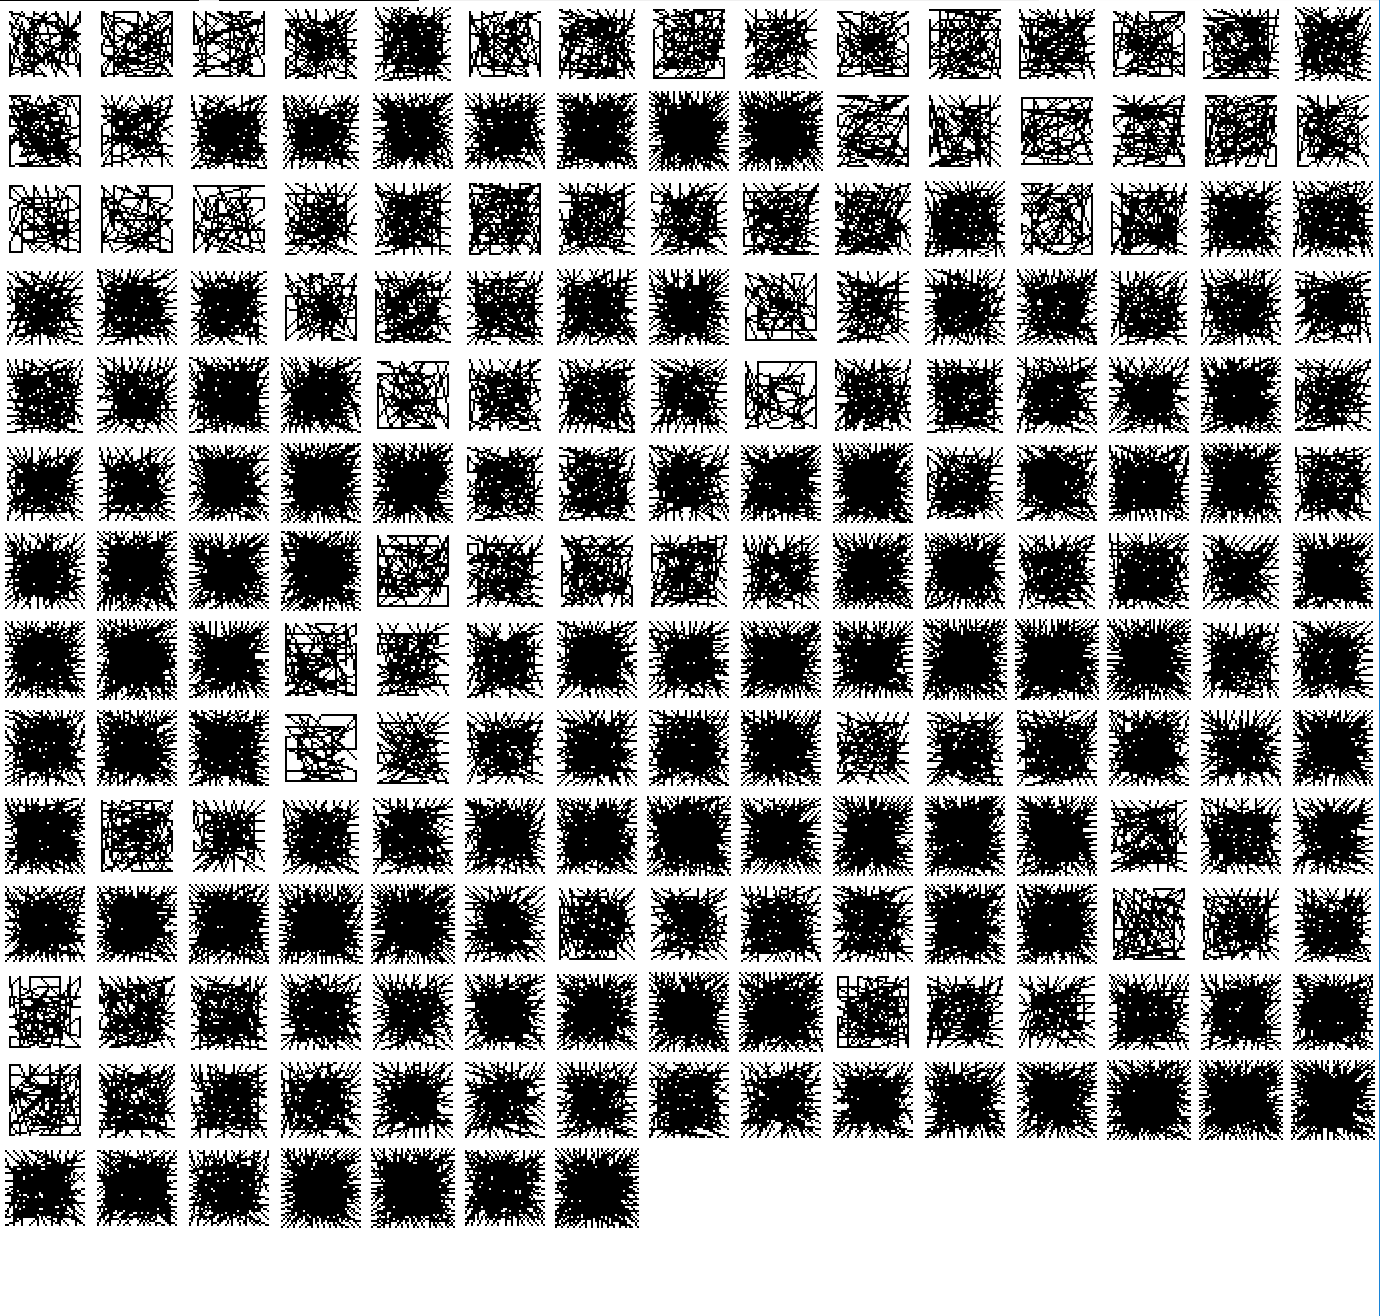
\includegraphics[width=0.5\textwidth]{img/ZilongLi2.png}}
                \subfigure[with crossing edges]{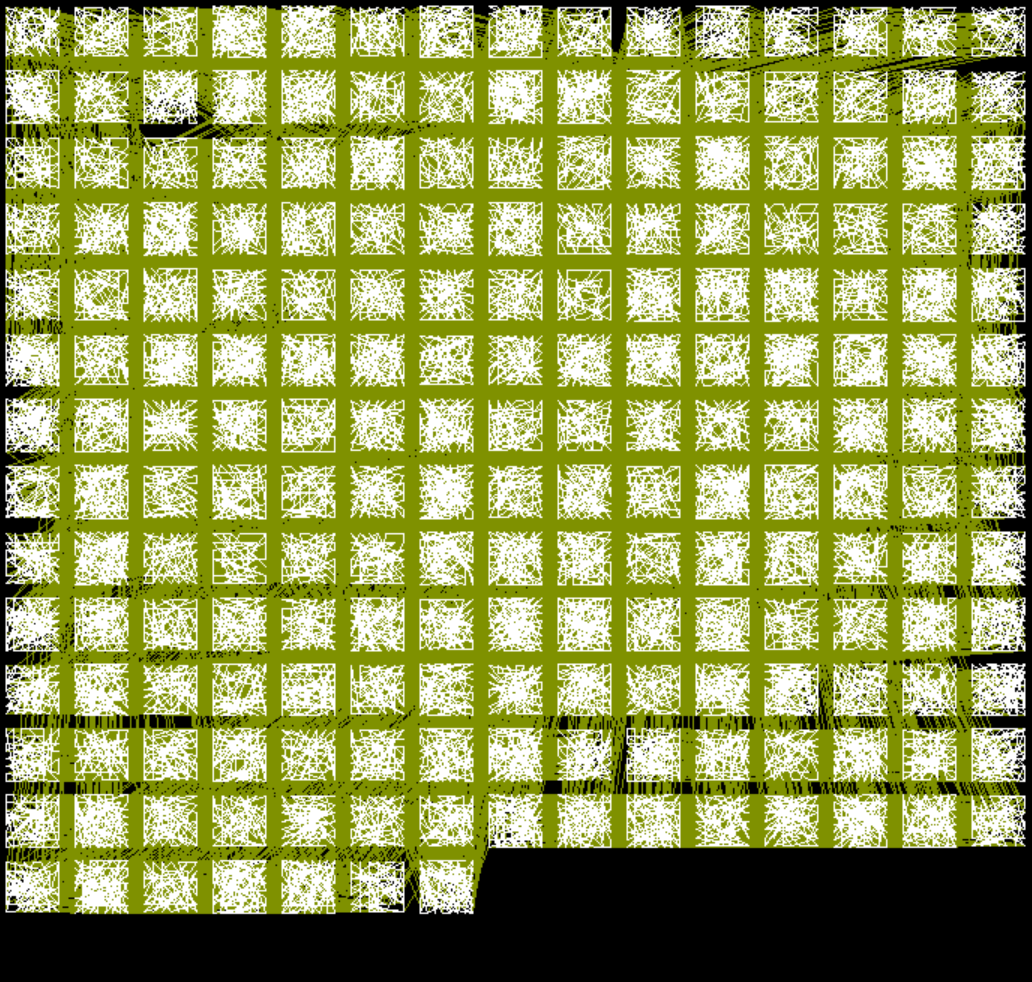
\includegraphics[width=0.5\textwidth]{img/ZilongLi3.png}}
                \caption{Using \href{https://github.com/LogCreative/GraphGenDecomp}{GraphGenDecomp}}
                \label{fig:ggd}
            \end{figure}
            
        \end{solution}
    \end{enumerate}	
\end{enumerate}

\begin{appendix}
\section{Code for Problem 4}
\fbox{\texttt{SCC.cpp}} is the main code for counting and getting the strong connected components. The additional output to \texttt{partition.txt} is for the input to GraphGenDecomp.
\begin{multicols}{2}
\lstinputlisting[language=c++]{SCC.cpp}
\end{multicols}
\fbox{\texttt{datapre.py}} is the data preprocessing code to adapt Gephi and GraphGenDecomp.
\begin{multicols}{2}
\lstinputlisting[language=python]{datapre.py}
\end{multicols}
\end{appendix}

\textbf{Remark:} Please include your .pdf, .tex, .cpp files for uploading with standard file names.
\newpage


%========================================================================
\end{document}
